
% Chapter 4 File

\chapter{Cubic Spline Interpolation and Theory}
\label{chapter3}
\thispagestyle{empty}

\section{Cubic Spline Definitions $\&$ Theorems}
We will continue by providing important definitions and theorems on cubic spline functions. First, we must establish a more rigorous definition of cubic spline interpolation.
\\\\
\emph{Definition 3.1.} Let $[a,b] \subset \mathbb{R}$. Then a \emph{partition} $P_n$ on $[a,b]$ is an ordered list of real numbers:
\\\\
\centerline{$ a=x_o < x_1 < x_2 < ... < x_{n-1} < x_{n}=b$}
\\\\
 Let $[a,b] \subset \mathbb{R}$, and let $P_n$ be a partition of $[a,b]$. A \emph{cubic spline} is a function $y \in C[a,b]$ such that $y|_{[x_{i}, x_{i+1}]}$ is a cubic polynomial.\newline
 \emph{Definition 3.2} We say that a function $g(x)$ \emph{interpolates} the data points $(x_i, y_i)$ for $i= 0,...,n$ when
\\\\
\centerline{$g(x_i)=y_i \hspace{4cm} \text{for} \ i=0,...,n$}
\\\\
\emph{Definition 3.3} We define the cubic spline space presented by Kreyszig as $S(K, P_{n})$ where $g$ is in $S(K, P_{n})$ if $g$ is a cubic spline on $P_n$ and $g \in C^2[a,b]$. \newline
\emph{Definition 3.4} We define the cubic spline space presented by Mhaskar-Pai as $S(MP, P_{n})$ where $g$ is in $S(MP, P_{n})$ if $g$ is a cubic spline on $P_{n}$ and $g \in C^1[a,b]$.
\\\\
Definition 3.2 tells us more about what cubic spline interpolation is and leads to the following theorems:
\\\\
\emph{Theorem 3.2.} \cite[pg.~358]{key3} Let $f(x)$ be a real-valued function on $[a,b]$. Define $P_{n}$ to be a partition of $[a,b]$ as referenced in Definition 1.3. Suppose $a_o, a_{n} \in \mathbb{R}$. Then there is a unique cubic spline function $g(x) \in S(K, P_{n})$ such that
\\\\
\centerline{(a) $g(x_{i})=f(x_{i})$} \newline
\centerline{(b) $g'(x_o)=a_o$} \newline
\centerline{(c) $g'(x_{n})=a_{n}$} \newline
for $i=0,1,...,n$. In particular, this holds if $f$ is differentiable and $a_{o} = f'(x_{o})$ and $a_{n} = f'(x_{n})$.
\\\\
\emph{Definition 3.5} \cite{key5} Here the Sobolev spaces $W^4_{p}[a,b]$ are subspaces of the Banach space $L^{p}[a,b]$ and include $C[a,b]$ as a subset.\\\\
\emph{Theorem 3.3} \cite[pg.~267]{key5} Let $f(x)$ be a real-valued function in $C[a,b]$. Define $P_{n}$ to be a partition of $[a,b]$ as referenced in Definition 1.3. Suppose $g(x) \in W^{4}_{2}$. Then there is a unique cubic spline function $g(x) \in S(MP, P_{n})$ such that
\\\\
\centerline{(a) $g(x_{i})=f(x_{i})$} \newline
\centerline{(b) $g'(x_{i})=f'(x_{i})$} \newline
for $i=0,1,...,n$.
\\\\
We will now introduce two error estimate theorems for cubic spline interpolants that are referenced in Mhaskar and Pai's \emph{Fundamentals of Approximation Theory} \cite[pg.~269]{key5}.
\\\\
\emph{Definition 3.6} Let $P_{n}$ be a partition.\newline Then we define $\|P_{n}\| = \sqrt{(x_{1}-x_{o})^2+(x_{2}-x_{1})^2+...+(x_{n}-x_{n-1})^2}$.\\\\
\emph{Theorem 3.4.} If $f \in W^{4}_{2}[a,b]$ and $I(f)$ is the unique cubic spline from theorem 3.2, then\\
$\|f-I(f)\|_{2} \leq (\frac{\|P_{n}\|}{\pi})^4\|f^{(4)}\|_{2}$.\\\\
\emph{Theorem 3.5.} If $f \in W^{4}_{\infty}[a,b]$, and $I(f)$ is the unique cubic spline from theorem 3.3 then\\
$\|f-I(f)\|_{\infty} \leq \frac{\|P_{n}\|^{4}}{384}\|f^{(4)}\|_{\infty}$.\\\\
This concludes the main definitions and theorems that we will be utilizing in answering our questions. To clarify how we find cubic splines, we will conclude this chapter with a practical example of using a cubic spline to approximate a function.

\section{Example of a Cubic Spline for $S(K, P_{n})$}
In this section, we will provide an example of finding a cubic spline in $S(K, P_{n})$. Let $f(x)=x^4$ be a function defined on the interval $[0,2]$ and let $P=\{0,1,2\}$ be the data points that partition the interval. It's one cubic spline with $2$ pieces. The piece $p_1$ will be defined on $[0,1]$ and the other denoted by $p_2$ on $[1,2]$. To find the $p_1$ and $p_2$ which are cubics, we will need to find $4$ coefficients for each, for a total of $8$ coefficients. Using Theorem 1.2 will result in the creation of $8$ conditions for finding the coefficients $a_{o},...,d_{1} \in \mathbb{R}$ for:\\\\
\begin{equation}
p(x) = \begin{cases}
p_1(x)= a_{o}x^3+b_{o}x^2+c_{o}x+d_{o} & \text{if } x \in [0,1]\\
p_2(x)= a_{1}x^3+b_{1}x^2+c_{1}x+d_{1} & \text{if } x \in [1,2]
\end{cases}
\end{equation}\\\\
We will need to satisfy the conditions:\\
$p_1(0)=f(0)$\newline
$p_1(1)=f(1)$\newline
$p_2(1)=f(1)$\newline
$p_2(2)=f(2)$\newline
$p_1'(0)=f'(0)$\newline
$p_2'(2)=f'(2)$\newline
$p_1'(1)=p_2'(1)$\newline
$p_1''(1)=p_2''(1)$\\\\
These conditions, when plugged into the equations for $p_1(x)$, $p_2(x)$, and $f(x)$, will result in a system of $8$ linear equations that can be solved via Gaussian elimination or through a computer program. A program in the Mathematica language is provided in Appendix A which can be used to find the coefficients. For this particular example, the cubic spline function for $f(x)$ is given by equation 3.2:\\\\
\begin{equation}
p(x) = \begin{cases}
p_1(x)=2x^3-x^2 & \text{if } x \in [0,1]\\
p_2(x)=6x^3-13x^2+12x-4 & \text{if } x \in [1,2]
\end{cases}
\end{equation}
\\\\
\section{Example of a Cubic Spline for $S(MP, P_{n})$}
In this section, we will provide an example of a cubic spline in $S(MP, P_{n})$. Let $f(x)=x^4$ be a function defined on the interval $[0,2]$ and let $P=\{0,1,2\}$ be the data points that partition the interval. The piece $p_1$ will be defined on $[0,1]$ and the other denoted by $p_2$ on $[1,2]$. To find the $p_1$ and $p_2$ which are cubics, we will need to find $4$ coefficients for each, for a total of $8$ coefficients. Using Theorem 1.2 will result in the creation of $8$ conditions for finding the coefficients $a_{o},...,d_{1} \in \mathbb{R}$ for:\\\\
\begin{equation}
p(x) = \begin{cases}
p_1(x)= a_{o}x^3+b_{o}x^2+c_{o}x+d_{o} & \text{if } x \in [0,1]\\
p_2(x)= a_{1}x^3+b_{1}x^2+c_{1}x+d_{1} & \text{if } x \in [1,2]
\end{cases}
\end{equation}\\\\
We will need to satisfy the conditions:\\
$p_1(0)=f(0)$\newline
$p_1(1)=f(1)$\newline
$p_2(1)=f(1)$\newline
$p_2(2)=f(2)$\newline
$p_1'(0)=f'(0)$\newline
$p_1'(1)=f'(1)$\newline
$p_2'(1)=f'(1)$\newline
$p_2'(2)=f'(2)$\\\\
Notice that in the Mhaskar-Pai algorithm there is an absence of the second derivative boundary condition and that none of the conditions interpolate the spline with the functions defined on each sub-interval. These conditions, when plugged into the equations for $p_1(x)$, $p_2(x)$, and $f(x)$, will result in a system of $8$ linear equations that can be solved via Gaussian elimination or through a computer program. A program in the Mathematica language is provided in Appendix A which can be used to find the coefficients. For this particular example, the cubic spline function for $f(x)$ is given by equation 3.4.\\\\
\begin{equation}
p(x) = \begin{cases}
p_1(x)=2x^3-x^2 & \text{if } x \in [0,1]\\
p_2(x)=6x^3-13x^2+12x-4 & \text{if } x \in [1,2]
\end{cases}
\end{equation}
\\\\
Notice that even though the interpolation conditions differ in both the Kreyszig and Mhaskar-Pai algorithms, the resulting spline $p(x)$ is the same. However, this is not always the case as sometimes the algorithms do not produce the same cubic spline. For example, consider the following spline functions approximating $\sin(x)$ on the partition $\{0,0.5,1,1.5,2\}$ with the first one resulting from using the Kreyszig algorithm and the second one resulting from using the Mhaskar-Pai algorithm:\\\\
\begin{equation}
p(x) = \begin{cases}
p_1(x)=-0.162107x^3-0.00124451x^2+x & \text{if } x \in [0,0.5]\\
p_2(x)=-0.123529x^3-0.0591105x^2+1.02893x-0.00482216 & \text{if } x \in [0.5,1]\\
p_3(x)=-0.0529067x^3-0.270979x^2+1.2408x-0.0754449 & \text{if } x \in [1,1.5]\\
p_4(x)=0.0295551x^3-0.642057x^2+1.79742x-0.353754 & \text{if } x \in [1.5,2]
\end{cases}
\end{equation}
\\\\
\begin{equation}
p(x) = \begin{cases}
p_1(x)=-0.160478x^3-0.00205866x^2+x & \text{if } x \in [0,0.5]\\
p_2(x)=-0.121188x^3-0.064608x^2+1.03308x-0.00581466 & \text{if } x \in [0.5,1]\\
p_3(x)=-0.052226x^3-0.273718x^2+1.24442x-0.0770009 & \text{if } x \in [1,1.5]\\
p_4(x)=0.0295224x^3-0.641877x^2+1.79709x-0.353557 & \text{if } x \in [1.5,2]
\end{cases}
\end{equation}
\\\\
\begin{figure}[htp]
    \centering
    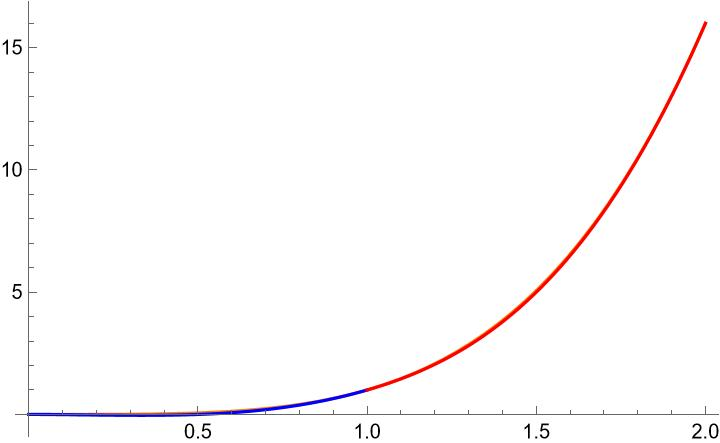
\includegraphics[width=150mm]{splinething.jpg}
    \caption{Graph of figures 3.2 and 3.4 with $p_1(x)$ (blue), and $p_2(x)$ (red).}
    \label{fig:spline_example}
\end{figure}
\\\\
\begin{figure}[htp]
    \centering
    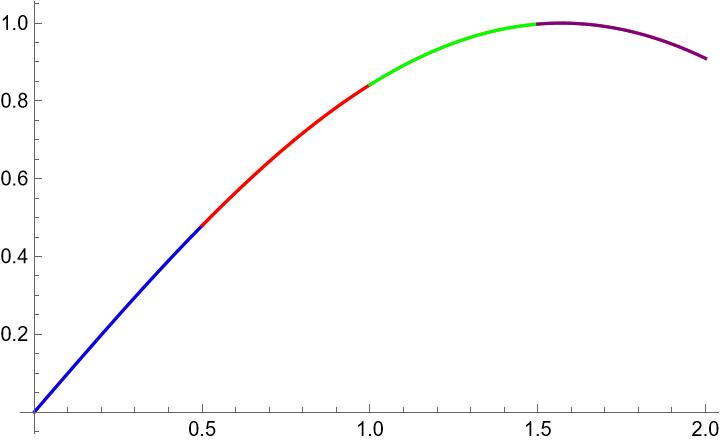
\includegraphics[width=150mm]{splinething2.jpg}
    \caption{Graph of figures 3.5 with $p_1(x)$ (blue), and $p_2(x)$ (red), $p_3(x)$ (green), and $p_4(x)$ (purple).}
    \label{fig:spline_example}
\end{figure}
\\\\
\begin{figure}[htp]
    \centering
    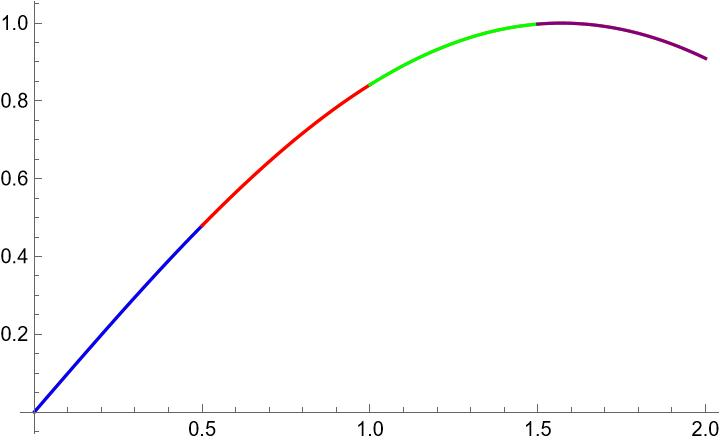
\includegraphics[width=150mm]{splinething3.jpg}
    \caption{Graph of figures 3.6 with $p_1(x)$ (blue), $p_2(x)$ (red), $p_3(x)$ (green) and $p_4(x)$ (purple).}
    \label{fig:spline_example}
\end{figure}